\documentclass[MTRX3700report.tex]{subfiles}
% Lydia
%\documentclass{article}
%\usepackage{graphicx}
%\usepackage{float}
%\usepackage{listings}

\begin{document}

\subsection{Module Requirements: Module IR sensors}
The Infrared Sensors module calculates the distance of the robot to the tilt and then determines whether this distance is either too close or too far away. THis module adheres to the following requirements:
\begin{enumerate}
	\item \textbf{Adjust sampling rate} according to the global variables 'IR Sample Rate' and 'IR Samples per Estimate' set by the user.
	\item \textbf{Calculate} the distance form the robot to the tilt in cm. 
	\item \textbf{Determine} whether the reading from the IR is out of range, and if so notify user that there is an error.	
	\item \textbf{Determine} whether the distance to the tilt is grater or lesser than a pre-defined set distance.
	\item \textbf{Output} raw reading from IR sensor and send to controller.
\end{enumerate} 

\subsubsection{Functional Requirements}
%This section describes the functional requirements of Module X – those requirements that must be met if the module (and system) is to function correctly. 
For this module to operate the following modules must first be initialized.
\begin{itemize}
	\item \textbf{Analog to Digital Converter} to sample reading from IR sensor.
	\item \textbf{Serial Communications} to send raw IR reading to controller.
\end{itemize}

\paragraph{Inputs}
%Describe each external input, including signal encoding and timing, message encoding and timing, protocols, file formats, protection against input errors, etc, as relevant.

The main input is the analogue signal from the IR sensor received through the Analogue to Digital converter on PORT A bit 1. 
The other inputs are the global variables 'IR Sample Rate' and 'IR Samples per Estimate' that determine the sampling rate of the IR sensor analogue signal and the number of samples to take before taking an average respectively. These variables can be changed by the user in Factory Mode through the controller.  

\paragraph{Process}
%Describe the internal signal transformations and/or computer processing functionality required within the module, required performance limits, and error tolerances as appropriate.

This modlue samples the value from the IR sensor continually through the use of an interrupt which triggers on the overflow of Timer 2. The Global variable 'IR Sample Rate' determines how many interrupts need to be triggered before taking a sample. Then the  Global variable 'IR Samples per Estimate' determines how many samples to take until the sample is finished.

When a sample is finished a function can be called which does the following in order:
\begin{enumerate}
	\item Calculate average of raw IR values. 
	\item Send this average value to the controller. 
	\item Check whether this value is within the IR senor range of 30cm.	
	\item If in range calculate distance in cm.
	\item Determine the state, whether there is an error or the distance is too close or too far.
\end{enumerate}
 
\paragraph{Outputs}
%Describe outputs that must be produced for the module to function correctly, including timing, frequency, protocols, etc as relevant.
This module produces three outputs:
\begin{itemize}
		\item The distance from the robot to the tilt in cm.
		\item The raw IR sensor value which is sent to the controller.
		\item The state of the system which controls the operation in auto mode. The states are error (when the IR sensor is out of range), too close and too far.
\end{itemize}
  
\paragraph{Timing}
%Any required timing or latency specifications that must be met.
The frequency that the Timer 2 overflow interrupt is triggered and therefore the sampling frequency of the IR sensor is determined by the frequncy of the PWMs for the motors discussed in its respective module. 

\paragraph{Failure Modes}
%Required functionality (if any) in the event of failure of various nominated components.
There is a chance of failure when the IR sensor is out of range. The range specified by the IR sensor datasheet is 4 to 30cm. When exceeding the range of 30cm this module outputs the state as error and does not calculate the distance in cm. 

However when the distance measured by the IR sensor is less than 4cm the state is determined not as an error but as too close. This is done to prevent the robot from stopping even if the distance from the robot to the tilt is less than 4cm. Although the distance output when this is the case will be incorrect.  

\subsubsection{Non-Function (Quality of Service) Requirements}
%Non-functional requirements do not need to be met for the device to have basic function, but are required to provide specific levels of performance or engineering quality.
\paragraph{Performance}
%Requirements such as computational loop time, accuracy, etc.
During Full Auto mode this module takes ost of the computational time. To reduce this time the following was implemented:
\begin{itemize}
	\item The interrupt only stores the raw IR values in a buffer and makes no calculations to reduce time spent in the interrupt to a minimum.
	\item The calculations on the raw IR values only start when a full sample is completed. This prevents doing the calculations multiple times for the same readings.
	\item The IR reading is checked to see if it is in range using the raw value to prevent the need to convert the value into cm (which is the most intensive part) when it is not in range. 
\end{itemize}
With the current frequency of the Timer 2 overflow interrupt the calculations can be completed before another full sample is made even when it takes a sample every interrupt for an average of one sample (ie. Global Variables 'IR Sample Rate' = 1,  'IR Samples per Estimate' = 1).

\paragraph{Interfaces}
%Requirements such as computational loop time, accuracy, etc.

The only part of this module directly interacting with the user is the output of the raw IR sensor value. This value is sent through serial communications once the average raw IR value is calculated once every full sample. Therefore the frequency that this value is sent is determined by the value of the global variables 'IR Sample Rate' and 'IR Samples per Estimate'. 

This value is large when the distance is short, and small when the distance is long. As this value can give the user no accurate indication of the current distance it should be used as a general indication of whether the IR sensor is working properly or not as well as a general approximation of the distance to the tilt.
 
\paragraph{Design Constraints}
%Practical or commercial considerations, such as programming languages, processor or other hardware, etc.
A major constraint to the design of this module was the use of the timer overflow interrupts. When testing on the PIC18F452 the timer 1 overflow interrupt was used with a defined pre-scaler making it possible to easily calculate the sampling rate for the IR sensors in Hz. However when integrating to the PIC18F4520 minimal board this interrupt along with the timer overflow interrupts for timer 0 and 3 would not work. The problem being unable to clear the interrupt flag. This forced us to use the timer 2 overflow interrupt with timer 2 being used in PWM mode for the motors.   

\subsection{Conceptual Design: Software Module IR Sensors}


\subsubsection{IR Sensors - an outline}
Once the IR sensors and interrupts are initialized this module continually samples values from the IR sensor. It is only when the user calls the function \textit{IR\textunderscore  Calculate} from the project main when a new distance will be calculated. Once the distance is calculated The resulting \textit{IR state} be it error, too close or too far can be used from the main to control the robot in Full Auto mode.

\subsubsection{Design Rationale}
This software module was designed so it could work as independently as possible from the other parts of the system. This was done through the header file \textit{IR\textunderscore Sensors.h} which gives the rest of the project access only to the following five functions:

\begin{itemize}
	\item char \textbf{Get\textunderscore S\textunderscore IR\textunderscore state}(void) - Returns a number 0 to 3 indicating as per the headers defines whether the current distance to the tilt is too close = 1, too far = 3 or error = 0.
	\item float \textbf{Get\textunderscore Current\textunderscore distance}(void) -  Returns the current distance as to the last call of IR\textunderscore Calculate in cm.  
	\item void \textbf{IR\textunderscore Setup}(void) - Setups the IR sensors. 
	\item void \textbf{IR\textunderscore  Sample}(void) - This function is made to be called from within a interrupt. It samples the IR sensor using an ADC and stors the values in a buffer. 
	\item void \textbf{IR\textunderscore  Calculate}(void) - This is the main function to be called from the main which calculates a new distance and state for the IR sensor. 
\end{itemize}

It was done in this manner to keep all the IR sensor functionality together in the one file \textit{IR\textunderscore Sensors.c}. This was especially important for the \textit{IR\textunderscore Sample} function which is used in an interrupt so all the interrupts for each module could be easily accessed and controlled from one file \textit{Interrupt\textunderscore Definition\textunderscore Robot.c}.



\subsubsection{IR calibration}
The IR sensor was calibrated using a tape measure and multimeter. The Voltage output of the sensor was recorded at different distances and then manipulated in EXCEL to generate an equation to convert the analog voltage output to distance in cm as shown below. 

\begin{figure}[h]
	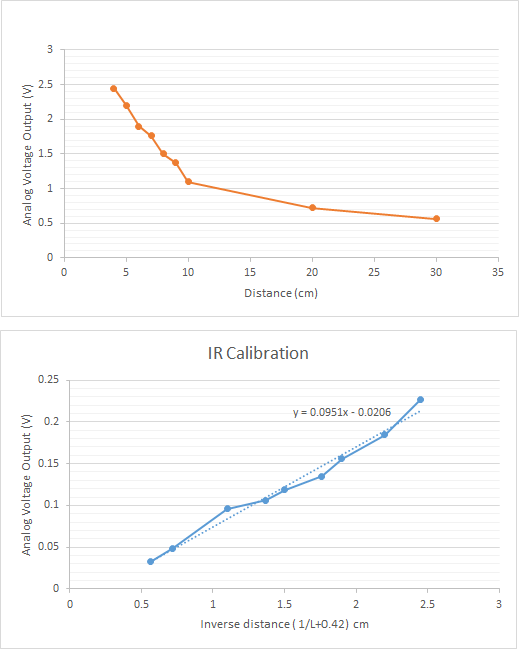
\includegraphics[scale=1]{IR_calibration.png}
	\centering
	\caption{EXCEL Calibration}
\end{figure}

This equation now had to be converted to take the voltage as a value between 0 and 255 as it is after going through an analog to digital conversion. The equation is as follows:

\begin{equation}
Distance (cm) = 1/((m*IRvalue*5/255)-b)-0.42
\end{equation}

Where m = 0.095 and b = 0.021 as calculated by excel

This equation was then hard-coded, meaning that the IR sensor could not be further calibrated without manually changing the code. This is not much of a problem as the accuracy of this distance is not so important to function correctly in Full Auto mode, as long as the results are consistent. 

\subsubsection{IR Flowcharts}

\begin{figure}[h]
	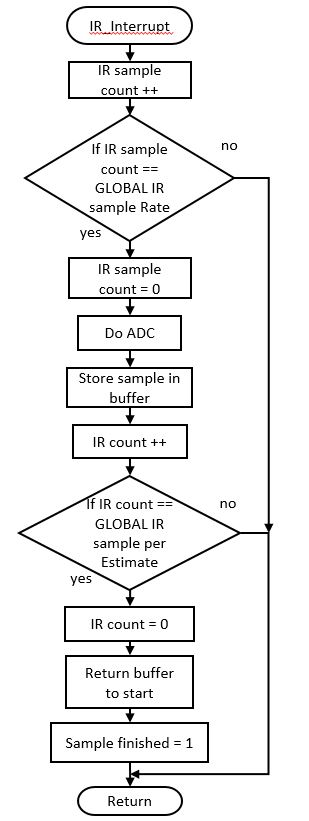
\includegraphics[scale=0.8]{IR_interrupt.jpg}
	\centering
	\caption{IR Interrupt Flowchart}
\end{figure}

\begin{figure}[h]
	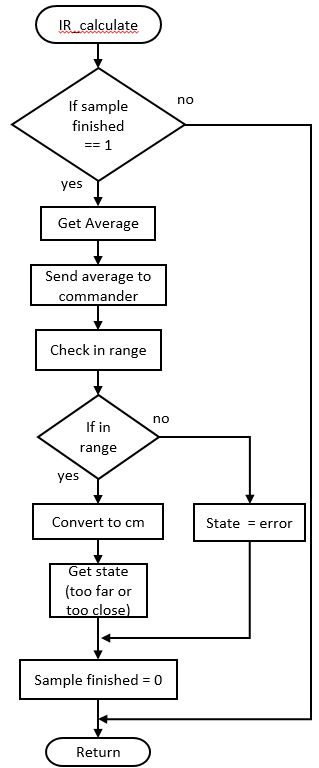
\includegraphics[scale=0.8]{IR_calculate.jpg}
	\centering
	\caption{IR Calculate Flowchart}
\end{figure}

\subsubsection{Assumptions Made}
The major assumption made was that run time efficiency was more important than the actula accuracy of the distance calculated. This is why the calibration was hard-coded in and why a linear equation was used for converting the value to cm instead of a polynomial equation.




\end{document}